\documentclass[a4paper, 12pt, twoside, openright]{book}
\usepackage[english,italian]{babel}
\usepackage[T1]{fontenc}
\usepackage[utf8]{inputenc}
\usepackage{fancyhdr}
\usepackage{float}
\usepackage{graphicx}
\usepackage{wrapfig}
\usepackage{siunitx} %per scrivere il simbolo °
\usepackage{verbatim} %per i commenti1
\usepackage{subfig}
\usepackage{amsmath}
\usepackage{algorithm}
\usepackage{algpseudocode}
\setcounter{secnumdepth}{3}
\setcounter{tocdepth}{6}
\usepackage{multirow}
\newcommand{\minitab}[2][l]{\begin{tabular}#1 #2\end{tabular}}
\usepackage{rotating}
\usepackage{xfrac}
\usepackage{enumitem}
\usepackage{amsmath}

\DeclareMathOperator*{\argmax}{arg\,max}
\DeclareMathOperator*{\argmin}{arg\,min}

%\usepackage{booktabs,array}
%\usepackage{tikz}

%\usepackage{tabularx}

%\usepackage{chngcntr}
%\counterwithin{table}{section}

%------------------------------ colors
\usepackage[usenames,dvipsnames,table]{xcolor} % use colors on table and more
\definecolor{333}{RGB}{51, 51, 51} % define custom color
\definecolor{background}{RGB}{255, 254, 213}
\definecolor{comment}{RGB}{17,167,5}
\definecolor{keyword}{RGB}{195,47,8}
\definecolor{string}{RGB}{142,195,0}
\definecolor{number}{RGB}{90,84,84}
\definecolor{identifier}{RGB}{0,90,201}

%------------------------------ source code
\usepackage{listings}

\lstset{
  basicstyle=\footnotesize\sffamily,
  commentstyle=\itshape\color{gray},
  captionpos=b,
  frame=shadowbox,
  language=HTML,
  rulesepcolor=\color{333},
  tabsize=2
}

\lstdefinestyle{code}{
  backgroundcolor=\color{background},
  basicstyle=\footnotesize\sffamily,
  commentstyle=\color{comment},
  frame=L,
  identifierstyle=\color{identifier},
  keywordstyle=\color{keyword},
  numbers=left,
  numbersep=10pt,
  numberstyle=\tiny\color{number},
  stringstyle=\color{string},
  showstringspaces=false,  
  stepnumber=1,
  tabsize=2
}


%------------------------------ define Abstract environment, missing in the 'book' class
\newenvironment{abstract}{\cleardoublepage \null \vfill \begin{center}\bfseries\abstractname \end{center}}{\vfill\null}
\addto\captionsenglish{\renewcommand*\abstractname{Abstract}} % change Abstract title

%------------------------------ active url
\usepackage{url}
\renewcommand{\UrlFont}{\color{black}\small\ttfamily}
\usepackage[colorlinks=true, linkcolor=black, citecolor=black, urlcolor=black]{hyperref} % active ref
%------------------------------ macros
\newcommand{\sectionname}{Section} % define Section ref
\newcommand{\subsectionname}{Sub-section} % define Sub-section ref
\renewcommand*\arraystretch{1.4} % tables padding

%acronimi
\usepackage[printonlyused]{acronym}

\begin{document}
\frontmatter

\begin{titlepage} %------------------------------ TITLE PAGE
\begin{center}

\hspace{0.5cm}
\begin{minipage}{.20\textwidth}
  
\includegraphics[height=2.5cm]{Images/UNIPD}
\end{minipage}\begin{minipage}{.90\textwidth}
  \begin{table}[H]
  \begin{tabular}{l}
  \scshape{\Large{\bfseries{Università degli Studi di Padova}}} \\
  \hline \\
  \scshape{\Large{Facoltà di Ingegneria}} \\
  \end{tabular}
  \end{table}
\end{minipage}

\vspace{1cm}
\emph{\Large{Corso~di~Laurea~Magistrale~in~Ingegneria~Informatica}} \\
\vspace{3cm}
\scshape{\Large{Tesina di Ricerca Operativa 2}} \\
\end{center}

\vspace{1cm}
\begin{center}
\scshape{\Large{\bfseries{Travelling Salesman}}}\\
\scshape{\Large{\bfseries{Problem}}}
\end{center}

\vspace{3.5cm}

\begin{center}
\emph{Autori}
\vspace{0.2cm}
\begin{table}[h]
\centering
\begin{tabular}{rl}
\vspace{0.2cm}
{Raffaele Di Nardo Di Maio} & {1204879}\\
{Cristina Fabris} & {1205722}\\
\end{tabular}
\end{table}

\end{center}

\vfill
\begin{center}
\hspace{-0.2cm}
\line(1, 0){360}\\
\textsc{Anno Accademico 2019-2020}
\end{center}
\end{titlepage}

%\begin{comment}
\begingroup %------------------------------ CONTENTS
  \makeatletter
  \let\ps@plain\ps@empty
  \makeatother
  \tableofcontents  
  \clearpage
\endgroup
%\end{comment}

\makeatletter
\def\@makechapterhead#1{%
  \vspace*{50\p@}%
  {\parindent \z@ \raggedright \normalfont
    \vskip 20\p@
    \interlinepenalty\@M
    \Huge \bfseries #1\par\nobreak
    \vskip 40\p@
  }}
\makeatother


\mainmatter
\chapter{Introduzione}\label{intro}
La seguente trattazione analizza il Problema del Commesso Viaggiatore (Travelling Salesman Problem, TSP), che consiste nell'individuare un circuito hamiltoniano di costo minimo in un assegnato grafo orientato G=(V,A)\cite{TSP}. La formulazione matematica di tale problema è la seguente:
$$
x_{ij}=
\begin{cases}
1 & se\;l'arco\;(i,j)\in A\;viene\;scelto\;nel\;circuito\;ottimo\\
0 & altrimenti\\
\end{cases}
$$
\begin{align}
& min \underset{(i,j)\in A}\sum{c_{ij}\;x_{ij}} \\\notag \\
& \underset{(i,j)\in \delta^{-}(j)}\sum{\;x_{ij}} = 1 & \forall\;j\in V \\\notag \\
& \underset{(i,j)\in \delta^{+}(i)}\sum{\;x_{ij}} = 1 & \forall\;i\in V \\\notag \\
& \underset{(i,j)\in \delta^{+}(S)}\sum{\;x_{ij}} \geq 1 & S \subset V\; :\; 1\in S\\\notag \\
& x_{ij}\geq 0\;\; intero & (i,j)\in A.\\\notag
\end{align}
Tuttavia le soluzioni algoritmiche presentante risolvono una sua variante, detta simmetrica, che viene applicata ad un grafo completo non orientato G=(V,E).\\ Di seguito viene riportata la formulazione matematica di tale versione:\\
\begin{align}
& min \underset{e\in E}\sum{c_e\;x_e}\\
& \underset{e\in \delta(v)}\sum{\;x_e} = 2 & \forall\;v\in V \\
& \underset{e\in E(S)}\sum{\;x_e} \leq \vert S\vert - 1 & \forall\;S\underset{\neq} \subset V: \vert S\vert\geq 3.\\\notag
\end{align}
A livello commerciale esistono diverse tipologie di risolutori di problemi di programmazione lineare intera, basati sul Branch \& Bound. I più conosciuti in circolazione sono i seguenti:
\begin{itemize}
\item{\textbf{IBM ILOG CPLEX Optimization Studio}\cite{ILOG}\\
è un soluzione analitica, sviluppata dall'IBM e gratuita a livello accademico.}
\item{\textbf{FICO® Xpress Optimization}\cite{FICO}\\
è stato prodotto dalla Fair Isaac Corporation(FICO) ed è costituito da 4 componenti principali: FICO® Xpress Insight, FICO® Xpress Executor, FICO® Xpress Solver e FICO® Xpress Workbench. Questa soluzione è disponibile gratuitamente solo nella versione Community, in cui però vengono applicate restrizioni sul numero di righe e colonne del tableau, di token non lineari e di funzioni dell'utente.}
\item{\textbf{Gurobi}\cite{GUROBI}\\
è una soluzione, sviluppata dalla Gurobi Optimization, che viene rilasciata anche con una versione accademica.}
\item{\textbf{COIN Branch and Cut solver (CBC)}\cite{CBC}\\
è un risolutore MIP(mixed-integer program) open-source scritto in C++ e sviluppato dalla Computational Infrastructure for Operations Researc (COIN).}
\end{itemize}
Nel Capitolo \ref{CPLEX} vengono riportate diverse soluzioni mat-euristiche e non per il problema del Commesso Viaggiatore, che fanno uso di ILOG CPLEX.\\
In commercio, il più noto ed efficiente software per la risoluzione del TSP è Concorde, sviluppato in ANSI C e disponibile per l'uso in ambito accademico\cite{concorde}.\\
Nel Capitolo \ref{HEURISTIC} vengono analizzati gli algoritmi euristici, sviluppati senza far uso di ILOG CPLEX.\\
Nel Capitolo \ref{PERF_PROF} vengono invece riportati i confronti, a livello temporale e di costo, delle soluzioni ottenute con i differenti algoritmi enunciati.\\
Nell'Appendice \ref{TSPlib}, \ref{CPLEX_func}, \ref{gnuplot}, \ref{perf_profile_py} vengono descritte rispettivamente la tipologia di istanze utilizzate, la documentazione utilizzata ed il funzionamento di CPLEX, il programma GNUPLOT utilizzato nella stampa delle soluzioni e il programma perfprof.py usato per creare i performance profile del Capitolo \ref{PERF_PROF}.\\
Tutti i tempi di esecuzione e i costi delle soluzioni, ottenuti mediante la fase di testing, sono consultabili invece nelle tabelle riportate nell'Appendice \ref{results}. Tutte le soluzioni descritte sono state implementate in linguaggio C e testate sul sistema operativo Windows 10 con Visual Studio, ed i sorgenti sono disponibili online\footnote{\url{https://github.com/RaffaDNDM/Operational-Research-2}}.
\chapter{Istanze e soluzioni del problema}
\section{Istanze}
Le istanze del problema, analizzate durante il corso, sono punti dello spazio 2D, identificati quindi da due coordinate ($x$,$y$).
Per generare istanza enormi del problema, si utilizza un approccio particolare in cui viene definito un insieme di punti a partire da un'immagine già esistente.\\
La vicinanza dei punti generati dipende dalla scala di grigi all'interno dell'immagine (es. generazione di punti a partire dal dipinto della Gioconda\cite{monnalisa}).\\
Le istanze che vengono elaborate dai programmi, creati durante il corso, utilizzano il template \textbf{TSPlib}. Di seguito viene riportato il contenuto di un file di questa tipologia.
 
\lstinputlisting[caption={\footnotesize{esempio.tsp}}, style=code, firstnumber=1, firstline=1, lastline=12, label=tsp_instance]{Source/esempio.tsp}

Le parole chiave più importanti, contenute in questi file \ref{tsp_instance}, sono:
\begin{itemize}
\item{\textbf{NAME}\\
seguito dal nome dell'istanza TSPlib}
\item{\textbf{COMMENT}\\
seguito da un commento associato all'istanza}
\item{\textbf{TYPE}\\
seguito dalla tipologia dell'istanza}
\item{\textbf{DIMENSION}\\
seguito dal numero di nodi nel grafo ($num\_nodi$)}
\item{\textbf{EDGE\_WEIGHT\_TYPE}\\
seguito dalla specifica del tipo di calcolo che viene effettuato per ricavare il costo del tour}
\item{\textbf{NODE\_COORD\_SECTION}\\
inizio della sezione composta di $num\_nodi$ righe in cui vengono riportate le caratteriste di ciascun nodo, nella forma seguente:
\begin{lstlisting}[linewidth=250pt,basicstyle=\footnotesize\sffamily,]     
indice_nodo  coordinata_x  coordinata_y
\end{lstlisting}}
\item{\textbf{EOF}\\
decreta la fine del file}
\end{itemize}

\section{Soluzioni}
Una soluzione del problema è una sequenza di nodi che corrisponde ad una permutazione dell'istanza (es. $S = \{x_1,x_2,...,x_n\}$ tale che $x_i=x_j\;\;x_i \in \Pi\;\forall\;x_i\in S\;\wedge\; x_i!=x_j\;\forall\;i\neq j$). Poichè in questa variante non esiste alcuna origine, ogni tour può essere descritto da due versi di percorrenza e l'origine può essere un nodo qualsiasi del grafo.
\subsection{Gnuplot}\label{gnuplot}
Una volta ottenuta la soluzione del problema di ottimizzazione, viene disegnato il grafo per facilitare all'utente la comprensione della sua correttezza. Per fare ciò viene utilizzato Gnuplot, un programma di tipo command-driven.\\
Per poterlo utilizzare all'interno del proprio programma esistono due metodi:
\begin{itemize}
\item{Collegare la libreria ed invocare le sue funzioni all'interno del nostro programma}
\item{Collegare l'eseguibile interattivo al proprio programma. In questo caso i comandi deve essere passati all'eseguibile attraverso un file di testo e l'utilizzo di un pipe.}\\
\end{itemize}
In questa trattazione è stato scelto il secondo metodo. All'interno del file è possibile specificare a Gnuplot le caratteristiche grafiche che deve aver il grafo. Di seguito viene riportato un esempio di tale file.\\

\lstinputlisting[caption={\footnotesize{style.txt}}, style=code, firstnumber=1, firstline=1, lastline=12, label=style_example]{Source/style_example.txt}

Nell'esempio sopra riportato, nella prima parte viene definito lo stile, il colore delle linee e la tipologia di punti, che verrano in seguito visualizzati all'interno del grafico prodotto.\\In seguito viene effettuato il plot del grafo in una finestra, utilizzando il primo e secondo valore di ciascuna riga del file \textbf{solution.dat} come coordinate mentre il terzo valore viene utilizzato come etichetta.\\\\
Il file \textbf{solution.dat} contiene le informazioni relative alla soluzione del grafico in cui ciascuna riga ha la seguente forma:
\begin{lstlisting}[linewidth=290pt,basicstyle=\footnotesize\sffamily,]     
coordinata_x   coordinata_y   posizione_in_tour
\end{lstlisting}
\textbf{coordinata\_x} rappresenta la coordinata x del nodo;\\
\textbf{posizione\_in\_tour} rappresenta la coordinata y del nodo;\\
\textbf{posizione\_in\_tour} rappresenta l'ordine del nodo all'interno del tour, assunto come nodo di origine il nodo 1.\\\\
Il grafico viene generato dal comando \textbf{plot}, leggendo tutte le righe non vuote e disegnando un punto nella posizione \textbf{(coordinata\_x,coordinata\_y)} del grafico 2D. In seguito viene tracciata una linea solo tra coppie di punti, legati a righe consecutive non vuote all'interno di \textbf{solution.dat}.\\\\
Attraverso le istruzioni riportate nelle righe 10-12 di \textbf{style.txt}, viene invece salvato il grafico appena generato nell'immagine \textbf{solution.png}.\\\\
Di seguito vengono riportate le varie fasi necessarie alla definizione di un pipe e al passaggio di questo al programma GNUplot:
\begin{itemize}
\item{\textbf{Definizione del pipe}
\lstinputlisting[style=code, firstnumber=1, firstline=1, lastline=1, label=style_example language=C]{Source/gnuplotC.txt}
dove \textbf{GNUPLOT\_EXE} è una stringa composta dal percorso completo dell'eseguibile di GNUplot, seguita dall'argomento \textbf{-persistent} (es. \textit{"D:/Programs/GNUplot/bin/gnuplot -persistent"}).
}
\item{\textbf{Passaggio delle istruzioni a GNUplot}
\lstinputlisting[style=code, firstnumber=2, firstline=2, lastline=10, label=style_example, language=C]{Source/gnuplotC.txt}
viene passata una riga alla volta, del file \textbf{style.txt}, a GNUplot mediante il pipe precedentemente creato.
}
\item{\textbf{Chiusura del pipe}
\lstinputlisting[style=code, firstnumber=11, firstline=11, lastline=11, label=style_example, language=C]{Source/gnuplotC.txt}
}
\end{itemize}
\chapter{CPLEX}

Per poter utilizzare gli algoritmi di risoluzione forniti da CPLEX è necessario costruire il modello del problema legato all'istanza sopra descritta.\\
CPLEX possiede due meccanismi di acquisizione del modello:

\begin{itemize}
\item{modalità interattiva: in cui il modello viene letto da un file precedentemente generato (\textit{model.lp})}
\item{definendo il modello attraverso le API del linguaggio C (o del linguaggio utilizzato per la scrittura del programma)}
\end{itemize}

Per memorizzare tale modello CPLEX utilizza due strutture dati:

\begin{itemize}
\item{ENV (enviroment): contiene i parametri necessari all'esecuzione}
\item{LP: contiene i dati degli elementi del modello}
\end{itemize}

%inserire immagine

Ad ogni ENV è possibile associare più LP, ma nel nostro caso ne sarà sufficiente uno solo.\\

Come prima cosa, per poter costruire il modello da analizzare, è necessario creare un puntatore alle due strutture dati necessarie a CPLEX.\\

\lstinputlisting[caption={\footnotesize{modelTSP.txt}}, style=code, firstnumber=1, firstline=27, lastline=29, label=tsp_model, language=c]{Source/modelTSP.txt}

La funzione alla riga 2 alloca la memoria necessaria e riempie la struttura con valori di default. Nel caso in cui non termini con successo memorizza un codice d'errore in \textit{\&errore}. La funziona invocata nella riga successiva, invece, associa la struttura LP all'enviroment che gli viene fornito. "TSP" sarà il nome del modello creato.\\
Al termine di queste operazioni il modello, riempirlo è stata costruita la seguente funzione:\\

\begin{lstlisting}[linewidth=250pt, basicstyle=\footnotesize\sffamily,]     
build_model(&instanza_problema, env, lp);
\end{lstlisting}

Viene aggiunta al modello una colonna alla volta con i costi dei vari archi, sfruttando \\

\begin{lstlisting}[linewidth=350pt, basicstyle=\footnotesize\sffamily,]     
CPXnewcols(env, lp, num_colonne, vettore_costi,
 vettore_lower_bound, vettore_upper_bound, dato_binario, 
 stringhe_nomi);
\end{lstlisting}

Questa funzione aggiunge \textit{num\_colonne} colonne con una sola invocazione, per far si che ne aggiunga una sola è necessario passargli l'indirizzo di \textit{vettore\_costi, vettore\_lower\_bound, vettore\_upper\_bound, dato\_binario, stringhe\_nomi} affinché li veda come array da un elemento e non come variabili.

Per poter inserire il primo vincolo del problema\\

$$
\underset{e\in \delta(v)}\sum{\;x_e} = 2\;\;\;\;\;\;\;\;\;\;\;\;\;\;\;\;\;\;\forall\;v\in V \\\\
$$
\\
viene sfruttata la funzione \\

\begin{lstlisting}[linewidth=350pt, basicstyle=\footnotesize\sffamily,]     
 CPXnewrows(env, lp, numero_righe, vettore_termini_noti,
  vettore_tipo_vincoli, NULL, stringhe_nomi);
\end{lstlisting}

Anche in questo caso è necessario seguire le stesse accortezze dell'analoga sopra descritta poiché inserisce \textit{numero\_righe} alla volta.\\
In questo modo si viene a creare una matrice in cui è presente il valore 1 se il nodo in questione appartiene al ramo nella colonna corrispondente, 0 altrimenti.\\
Per convenzione è stato deciso di indicare tutti i rami $(i,j)$, con $i\neq j$, rispettando la proprietà $i<j$. Per tener conto di questo particolarità è necessario fare particolare attenzione nell'inserimento delle righe.\\

\begin{figure}[h!] 
\begin{center} 
  % Requires \usepackage{graphicx} 
  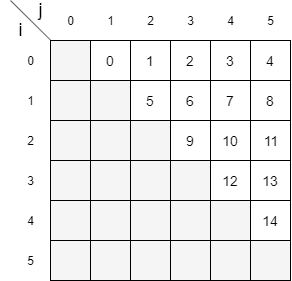
\includegraphics[width=14cm]{Images/indices_matrix}\\ 
  \caption{} 
\end{center} 
\end{figure}


%inserire immagine




\begin{thebibliography}{1}

\begin{comment}
\bibitem{alg} Pierluigi Crescenzi, Pierre Fraigniaud, Magnus Halldórsson, Hovhannes A. Harutyunyand, Chiara Pierucci, Andrea Pietracaprina, Geppino Pucci \emph {On the complexity of the shortest-path broadcast problem, Discrete Applied Mathematics , vol. 199, pp. 101-109, 2016.}
\end{comment}

\bibitem{cook} \emph{\url{http://www.math.uwaterloo.ca/tsp/}}

\bibitem{concorde} \emph{\url{http://www.math.uwaterloo.ca/tsp/concorde/index.html}}

\bibitem{monnalisa} \emph{\url{http://www.math.uwaterloo.ca/tsp/data/ml/monalisa.html}}

\bibitem{salvagnin_perf} Dolan, E. D., Mor{\'e}, J.J., \emph{Benchmarking optimization software with performance profiles}, Mathematical Programming, vol. 91, n. 2, pp. 201--213, 2002, Springer


\end{thebibliography}

\end{document}